%
\section{TS1 window}

Negative pions produced in antiproton annihilation at TS3 are a source
of ``delayed RPC'', negative pion captured happening significantly later
within the microbunch than capture of pions produced at the PT. 

TS1 antiproton window reduces the overall flux of protons entering the TS.
It is made of aluminum and its nominal thickness is 250 $\mu$.
As shown in Figure~\ref{figure:760_1300_vs_760_1000_ts4},
reducing the thickness of the TS1 window down to 50 $\mu$ Al results in the
increase of the delayed RPC background.

For T>700:

\begin{itemize}
\item
  TS3: 50 um Ti window + 6 127un thick Al strips 
\item
  background increases from $4 \cdot 10^{-3}$ to $2.5 \cdot 10^{-2}$
  in 3 years of running in 2 batch mode \cite{MU2E_33410_MURAT}
\end{itemize}

\begin{figure}
  \begin{tikzpicture}
    \node[anchor=south west,inner sep=0] at (0,0.) {
      % \node[shift={(0 cm,0.cm)},inner sep=0,rotate={90}] at (0,0) {}
      \makebox[\textwidth][c] {
        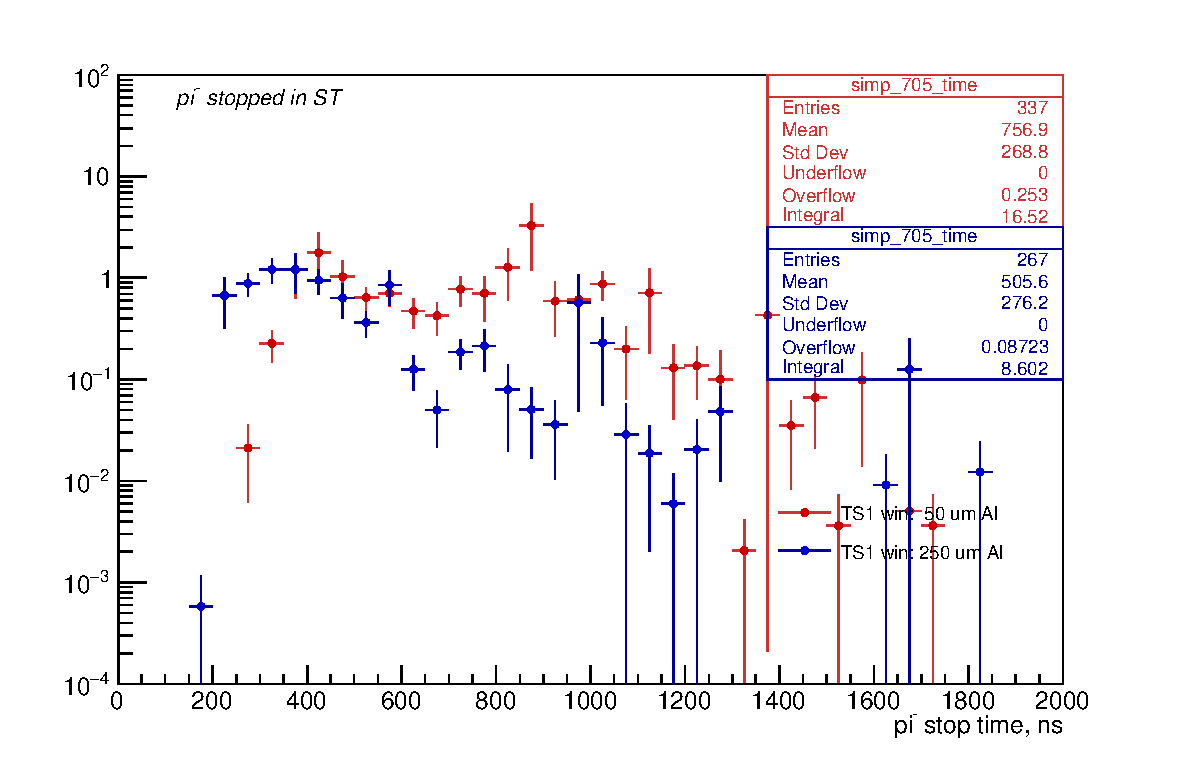
\includegraphics[width=0.8\textwidth]{figures/pdf/760_1300_vs_760_1000_ts4_tgtstops_simp_705_time}
      }
    };
    % \node [text width=6cm, scale=0.8] at (4.5,6.4) {mu2e-18894 by Kevin Lynch and Jim Popp};
  \end{tikzpicture}
  \caption{
    \label{figure:760_1300_vs_760_1000_ts4}
    aaa
  }
\end{figure}
%%% Local Variables:
%%% mode: latex
%%% TeX-master: t
%%% End:
